\subsection{Período $T$ en Función de $B$}

Según \cite{Grebogi1988}, el período $T$ se relaciona con la precisión $\epsilon$ como $T \sim \epsilon^{-d/2}$ donde $d$ es la dimensión de correlación del atractor caótico.
La evolución del período como función de la precisión para los mapas que se muestran aquí se informó en \cite{Nagaraj2008}.
Allí mostraron que el período $T$ del mapa compuesto obtenido al conmutar entre dos mapas caóticos es más alto que el período de cada mapa y encontraron que una conmutación aleatoria mejora los resultados.
Aquí hemos considerado el solo la conmutación secuencial para evitar el uso de otra variable aleatoria, ya que esta puede introducir sus propias propiedades estadísticas en la serie temporal.

La Figura \ref{fig:period} muestra $T$ vs. $B$ en escala semi logarítmica para el mapa LOG.
Para cada presición, se generararon 100 surrogados diferentes, cada uno con una condición inicial generada aleatoriamente.
La Figura muestra 100 puntos rojos por cada precisión de punto fijo ($1 \geq B \geq 53$) y los resultados promediados (puntos negros conectados con líneas entrecortadas negras).
Los puntos promediados experimentales se pueden ajustar por una línea recta expresada como $\log_2 T = mB + b$ donde $m$ es la pendiente y $b$ es la ordenada al origen.
%
\begin{figure}[htpb]
\centering	
	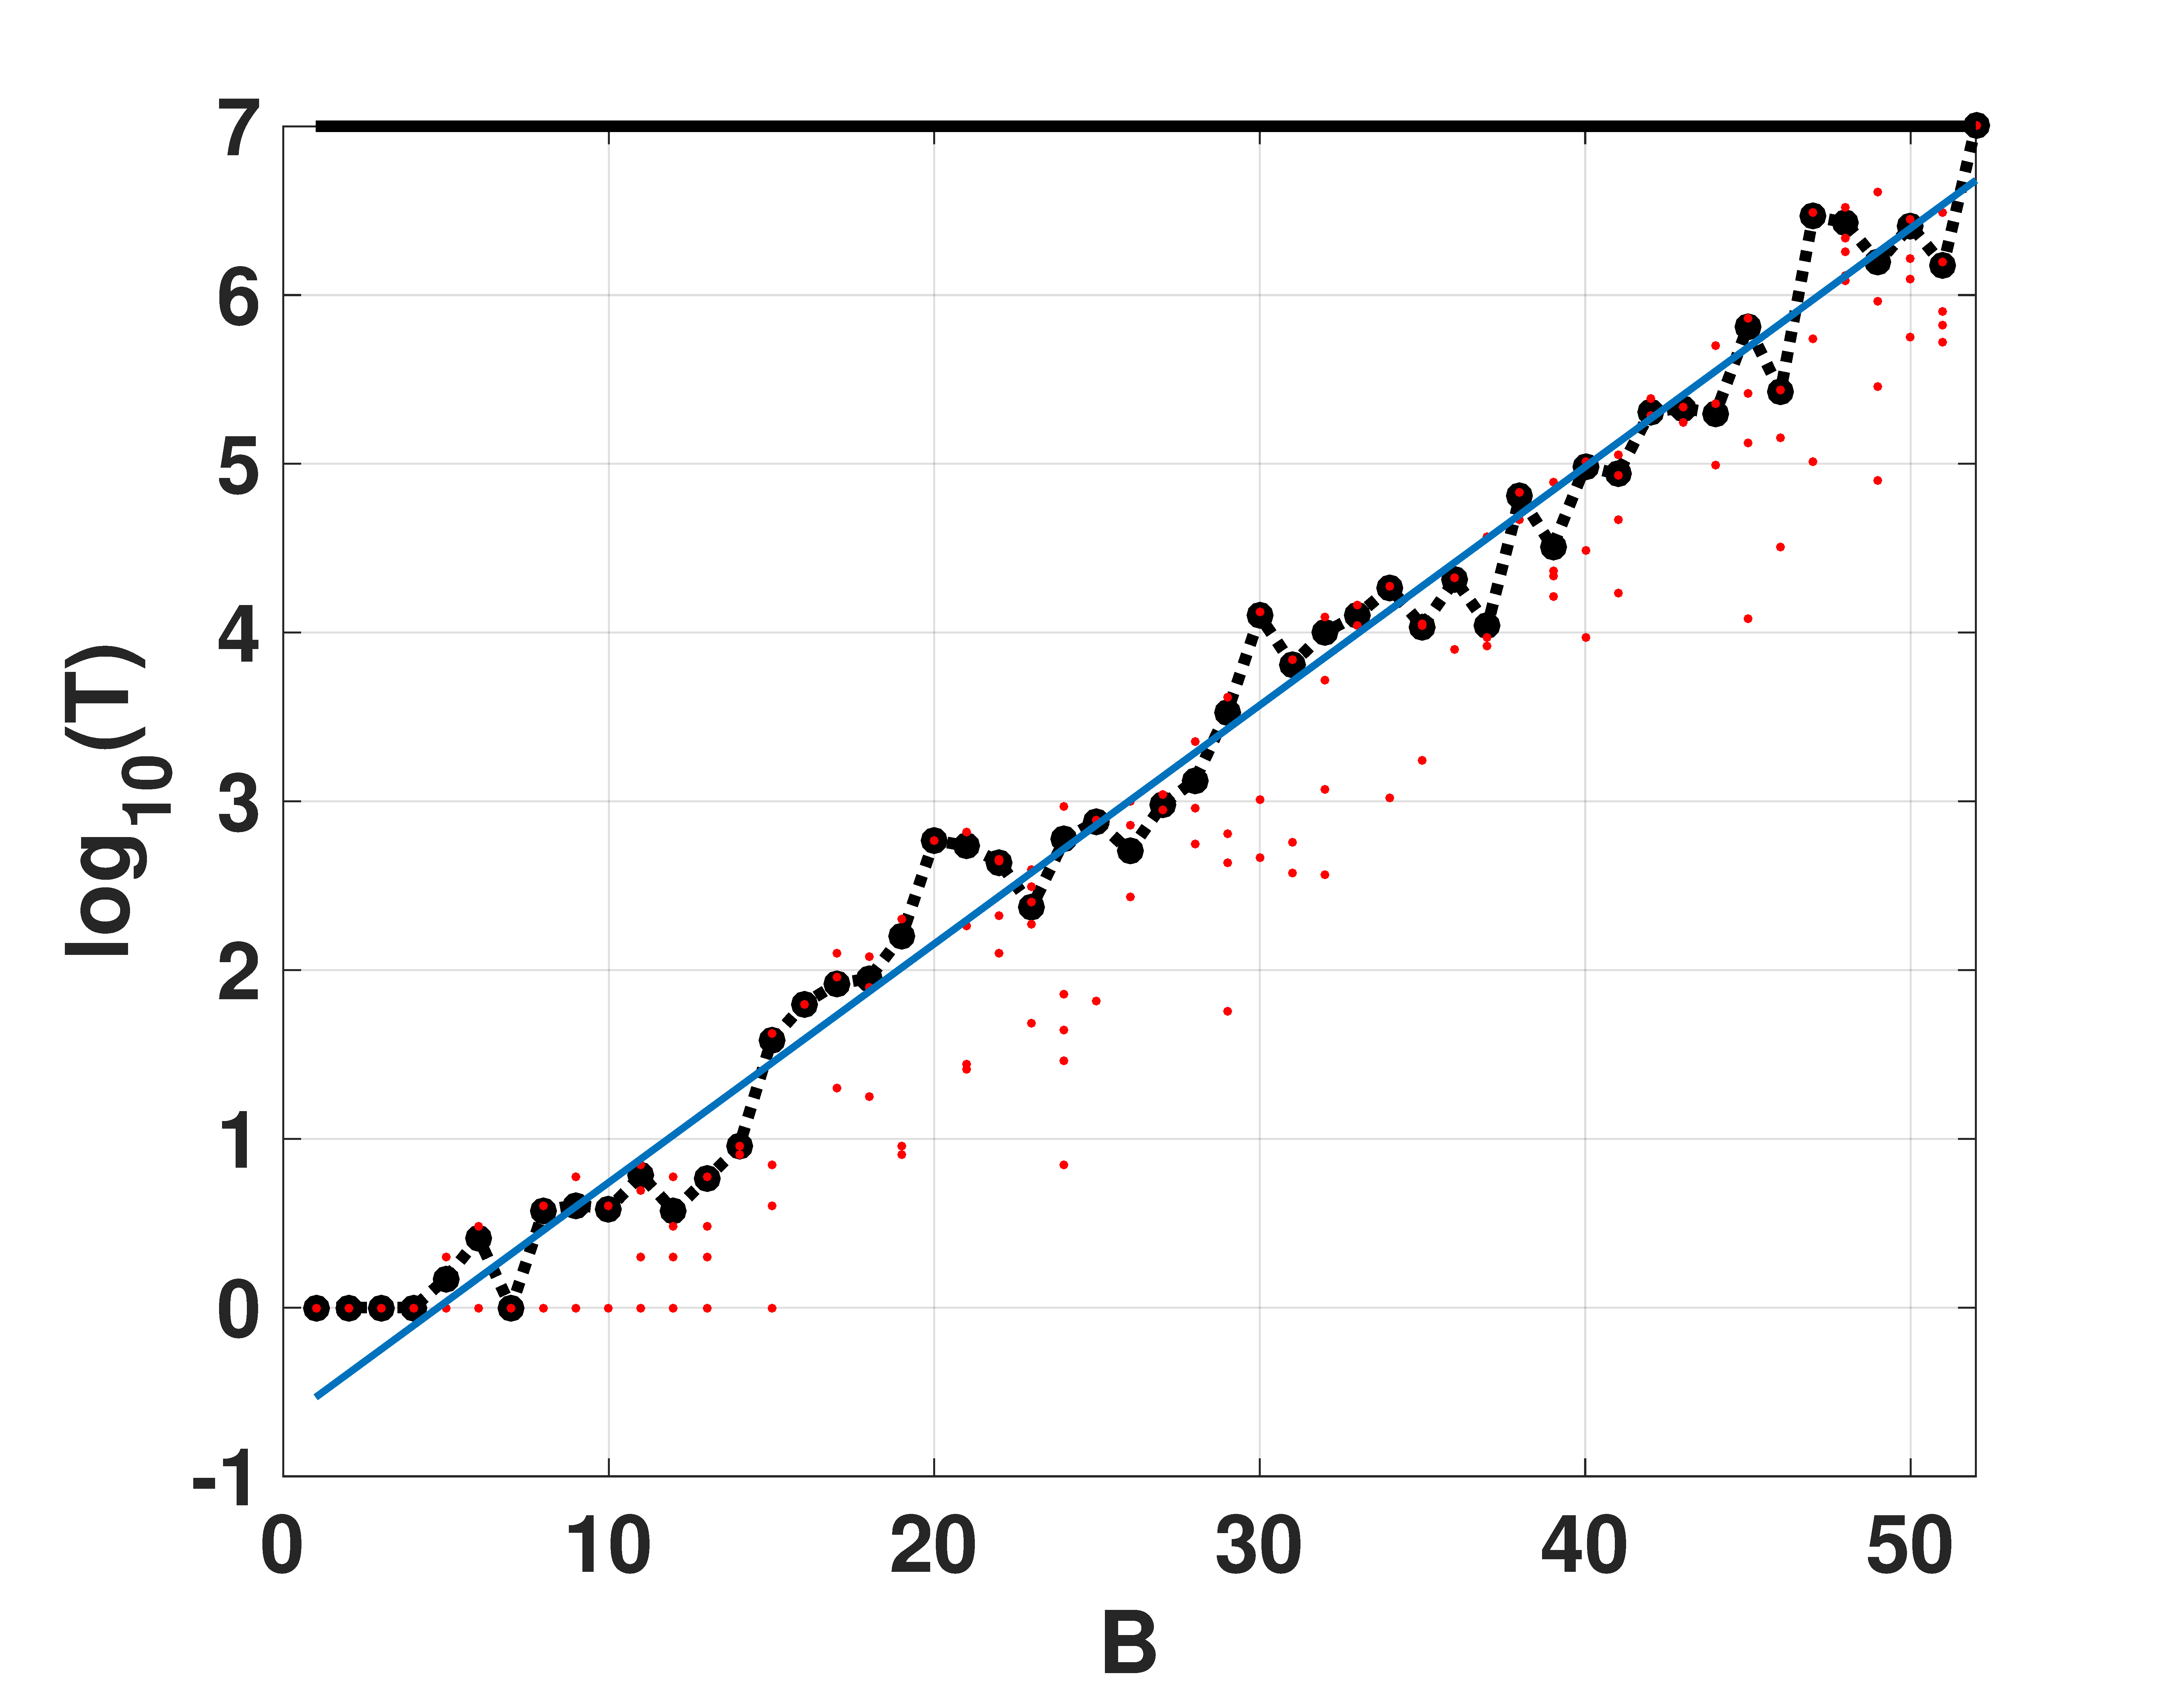
\includegraphics[width=.49\textwidth]{Period_Log}
	\caption{Período $T$ en función de la preceisión $B$ en números binarios para el mapa LOG.} \label{fig:period}
\end{figure}

Los resultados para todos los mapas considerados se resumen en el Cuadro \ref{tabla:periodos}.
Pudimos detectar que el período promediado fue el mismo usando $u=2$ y $u=1.96$ cuando se utiliza la estrategia de switching.
Por lo tanto para calcular los resultados mostrados en el Cuadro para SWITCH, EVEN y ODD se iteró con $u=2$.
%
\begin{table}[htpb]
	\centering	
	\caption{Período $T$ en función de la precisión $B$ para todos los mapas considerados. SWITCH, EVEN y ODD fueron calculados con $u=2$.}
	\vspace{1em}
	\begin{tabular}{lll}
		\hline\noalign{\smallskip}
		map 			& m 	& b  \\
		\noalign{\smallskip}\hline\noalign{\smallskip}
		TENT $u=2$		&0 		& 0 \\
		TENT $u=1.96$ 	&0.1487 & -0.01177 \\
		LOG 			&0.139 	& -0.6188 \\
		SWITCH 			&0.1462 & -0.5115 \\
		EVEN 			&0.1447 & -0.7783 \\
		ODD 			&0.1444 & -0.7683 \\
		\noalign{\smallskip}\hline
	\end{tabular}
	\label{tabla:periodos}	
\end{table}

Los resultados son compatibles con los obtenidos en \cite{Nagaraj2008}.
La conmutación entre mapas aumenta el período $T$ pero el procedimiento de skipping lo disminuye casi a la mitad.
Se puede observar que, los resultados para el mapa TENT con $u=1,96$ exhibe los mejores resultados.